%%%%%%%%%%%%%%%%%%%%%%%%%%%%%%%%%%%%%%%%%%%%%%%%%%%%%%%%%%%% 
% This is the official template for theses and seminar papers from the Chair for Information Systems for Sustainable Society (IS3) at the University of Cologne

%
%PREAMBLE
%%%%%%%%%%%%%%%%%%%%%%%%%%%%%%%%%%%%%%%%%%%%%%%%%%%%%%%%%%%%%

\documentclass[a4paper, 12pt]{article}
\usepackage[utf8]{inputenc}
\usepackage[T1]{fontenc}
\usepackage{graphicx}
\usepackage{longtable}
\usepackage{hyperref}
\usepackage{caption}
\usepackage{float}
\usepackage{psl-cover}


% set margins for double-sided printing
\usepackage[left=1cm, right=2.5cm, top=2.5cm, bottom=3cm, bindingoffset=1.5cm, head=15pt]{geometry} 
\usepackage{setspace}
\onehalfspacing
% set headers
\usepackage{fancyhdr}
\pagestyle{fancy}
\fancyhead{}
\fancyfoot{}
\fancyhead[LE,RO]{\textsl{\leftmark}}
\fancyhead[RE,LO]{\thesisauthor}
\fancyfoot[C]{ \\
\thepage}
\renewcommand{\headrulewidth}{0.4pt}
\renewcommand{\footrulewidth}{0.4pt}


% set APA citation style
\usepackage{apacite}
\usepackage[numbib,notlof,notlot,nottoc]{tocbibind}
\pagenumbering{gobble}

%%%%%%%%%%%%%%%%%%%%%%%%%%%%%%%%%%%%%%%%%%%%%%%%%%%%%%%%%%%%%
%THESIS Parameters 
%%%%%%%%%%%%%%%%%%%%%%%%%%%%%%%%%%%%%%%%%%%%%%%%%%%%%%%%%%%%%

\title{AVANCEMENT DE THÈSE
- Validation de 1ère année -
\\
Analyse des mouvements et gestes des piétons via caméra embarquée pour la prédiction de leurs intentions}

%%%%%%%%%%%%%%%%%%%%%%%%%%%%%%%%%%%%%%%%%%%%%%%%%%%%%%%%%%%%%
%DOCUMENT
%%%%%%%%%%%%%%%%%%%%%%%%%%%%%%%%%%%%%%%%%%%%%%%%%%%%%%%%%%%%%

\begin{document}



\author{Joseph Gesnouin}
\date{X Avril 2020}
\jurymember{5}{Fabien Moutarde}{Professeur, Mines ParisTech}{Directeur de thèse}
\jurymember{4}{Bogdan Stanciulescu}{Maître de conférences, Mines ParisTech}{Maitre de thèse}
\jurymember{3}{Steve Pechberti}{Ingénieur de recherche, Vedecom}{Encadrant industriel}

\jurymember{2}{Examinateur 2}{Titre}{Jury}
\jurymember{1}{Examinateur 1}{Titre}{Jury}

%% commandes avec des valeurs par défaut non nulles
%%\institute{nom de l’organisme d’accueil PSL}
\doctoralschool{Ingénierie des Systèmes, Matériaux, Mécanique, Energétique}{621}
\specialty{Informatique temps réel, robotique et automatique.}


\maketitle{}
%%%%%%%%%%%%%%%%%%%%%%%%%%%%%%%%%%%%%%%%%%%%%%%%%%%%%%%%%%%%%
%TITLE PAGE (Pre-defined, just change parameters above)
%%%%%%%%%%%%%%%%%%%%%%%%%%%%%%%%%%%%%%%%%%%%%%%%%%%%%%%%%%%%%
%\input{Template/Title.tex}

%\newpage
%\thispagestyle{empty}
%\strut
%\markboth{}{}
%\newpage

%%%%%%%%%%%%%%%%%%%%%%%%%%%%%%%%%%%%%%%%%%%%%%%%%%%%%%%%%%%%%
%Résumé
%%%%%%%%%%%%%%%%%%%%%%%%%%%%%%%%%%%%%%%%%%%%%%%%%%%%%%%%%%%%%
%
\vspace*{2.5cm}
\noindent\rule[2pt]{\textwidth}{0.5pt}\\
{\textbf{Résumé ---}}
Dans le cadre d’un pivot stratégique d’une entreprise de télécommunication à une entreprise numérique, l’analyse des données récupérées sur les équipements de l’univers résidentiel client permet l’analyse et l’amélioration de la qualité des services Orange. Directement rattaché à l’entité Groupe, le département DAQE (Data Analytics and Qs Enablers) fournit aux domaines d'activité stratégique des moyens de collecte et d’analyse des données des équipements maison. Durant mon apprentissage au sein de ce service, j’ai eu l’opportunité de comprendre l’ensemble de la chaîne de collecte et d’analyse des données à l'aide de technologies Big Data Orange, de mettre en pratique mes savoirs et techniques pour comprendre un environnement complexe et y développer de nouvelles briques de calcul. Pour finir, de nombreuses missions de veilles technologiques et de formations m’ont permis d’apprendre de nouvelles notions et des compétences de communication et d’organisation nécessaires au métier de data scientist.


{\textbf{Mots clés :}}
Data Mining, Chaine de collecte, Big Data, Analyse factorielle, Réseaux bayesiens, Inférence Causale, Apprentissage supervisé, Asymétrie, Livebox, Décodeur TV, Satisfaction Client, QoS.
\\
\noindent\rule[2pt]{\textwidth}{0.5pt}
\begin{center}
  Centre Universitaire des Saints-Pères, Université Paris Descartes \\
  45 Rue des Saints-Pères\\
  75006 Paris
\end{center}




%\newpage
%\thispagestyle{empty}
%\strut
%\markboth{}{}
%\newpage
%%%%%%%%%%%%%%%%%%%%%%%%%%%%%%%%%%%%%%%%%%%%%%%%%%%%%%%%%%%%%
%Confidentialité
%%%%%%%%%%%%%%%%%%%%%%%%%%%%%%%%%%%%%%%%%%%%%%%%%%%%%%%%%%%%%
%\clearpage
\section*{Note de confidentialité}
\label{sec:SOOA}

\vspace{1cm}
Ce document et son contenu sont de la propriété d’ORANGE. Aucun droit de propriété intellectuelle n’est accordé par la communication du présent document ou de son contenu. Ce document ne doit pas être reproduit ou communiqué à un tiers sans l’autorisation écrite d’ORANGE. Ce document et son contenu ne doivent pas être utilisés à d’autres fins que celles qui sont autorisées.
\vspace{1cm}

\textbf{\thesisauthor{}} 

\vspace{0.5cm}
\noindent
Guyancourt, le 10.06.2019


%\newpage
%\thispagestyle{empty}
%\strut
%\markboth{}{}
%\newpage
%%%%%%%%%%%%%%%%%%%%%%%%%%%%%%%%%%%%%%%%%%%%%%%%%%%%%%%%%%%%%
%Remerciements
%%%%%%%%%%%%%%%%%%%%%%%%%%%%%%%%%%%%%%%%%%%%%%%%%%%%%%%%%%%%%
%\clearpage
\section*{Remerciements}
\label{sec:remerciements}


\vspace{0.5cm}



\vspace{0.5cm}

\vspace{0.5cm}


\vspace{0.5cm}


\newpage
\thispagestyle{empty}
\strut
\markboth{}{}
\newpage

\vspace{0.5cm}


\vspace{0.5cm}


\vspace{0.5cm}

\vspace{3cm}
\noindent
\textbf{Joseph} 

\newpage
\thispagestyle{empty}
\strut
\markboth{}{}


%\thispagestyle{empty}
%\strut
%\markboth{}{}
%\clearpage
%\vspace*{\fill}
%\thispagestyle{empty} % optional -- suppress showing of page number
%\begin{quotation}
%\em % optional -- to switch to emphasis (italics) mode
%\medskip
%%\raggedleft
%"Je crois que la science\\ avec conscience et sans orgueil est le seul outil d'émancipation personnelle en premier lieu, collégiale sinon collective en second lieu" - Jean-Yves G.\\
%D'après Rabelais, Elysée Reclus, Primo Levi, Illiouchine, Bourdieu et Pascal.
%\end{quotation}
%\vspace*{\fill}

%\newpage
%\thispagestyle{empty}
%\strut
%\markboth{}{}
%\newpage





%%%%%%%%%%%%%%%%%%%%%%%%%%%%%%%%%%%%%%%%%%%%%%%%%%%%%%%%%%%%%
%TOC,TOF,TOT
%%%%%%%%%%%%%%%%%%%%%%%%%%%%%%%%%%%%%%%%%%%%%%%%%%%%%%%%%%%%%
%\clearpage
\pagenumbering{Roman}
\tableofcontents
\clearpage
\listoffigures
\clearpage
\listoftables
\clearpage

\pagenumbering{arabic}


%%%%%%%%%%%%%%%%%%%%%%%%%%%%%%%%%%%%%%%%%%%%%%%%%%%%%%%%%%%%%
%MAIN PART
%%%%%%%%%%%%%%%%%%%%%%%%%%%%%%%%%%%%%%%%%%%%%%%%%%%%%%%%%%%%%

% Introduction
\clearpage
\section{Introduction}
\label{sec:Intro}

\subsection{Contexte}
Cette thèse est réalisée au sein de l’unité “\textit{PELOPS}” (\textit{PErception LOcalization and Planning Systems for automated driving}) de l'institut Vedecom. Le laboratoire partenaire pour cette thèse est le Centre de Robotique de l'école Mines ParisTech. Le sujet d’étude concerne le lien entre la posture et l’attitude de marche afin d’en inférer des comportements. L’approche envisagée considère de l’apprentissage profond pour venir lier la position des articulations d’un piéton à une intention. L’objectif à l’issue de ces travaux est d’avoir une caractérisation de la trajectoire à venir du piéton afin d’aider à la prise de décision côté véhicule autonome.

\subsection{Sujet de thèse}
L'objectif de la thèse est d'étudier les méthodes basées sur les caméras pour prévoir les actions futures et les intentions des piétons dans un environnement de circulation urbaine.\\

L'objectif sera de définir une solution exploitant l’information caméra (domaine image) et reposant sur les réseaux de neurones pour concevoir un système capable de comprendre l’intention d’un piéton en fonction de sa gestuelle (dynamique du squelette), d'indicateurs contextuels (téléphone portable, ...) et de son environnement (route / trottoir, ...) puis d’en inférer la localisation future du piéton de manière à déterminer s’il est susceptible de représenter un obstacle pour le véhicule autonome ou non.

Nous définissons l'intention comme une combinaison de comportements discrets de haut niveau ainsi que de trajectoires continues décrivant le mouvement futur attendu du piéton. L’approche considérée serait donc capable de prédire les intentions des piétons sous forme discrète et continue : 

\begin{itemize}
    \item \textbf{Actions de haut niveau} : La prédiction de l'intention discrète peut être considérée comme une classification multi-classes : \textit{Crossing / Not Crossing / About to Cross / Waiting ...}
    \item \textbf{Régression de la trajectoire} : Pour chaque piéton, nous considerons sa trajectoire comme étant une séquence de bounding box, comprenant alors les emplacements actuels et futurs du dit piéton.
\end{itemize}

Les deux facteurs principaux envisagés pour réaliser ce travail sont les suivants :

\begin{itemize}
    \item  \textbf{Le piéton} : étant donné que les informations sur le positionnement de son mouvement, sa disposition physique et l'orientation de certains membres déterminent ce qu'un conducteur utilise communément pour en déduire sa position future.
    \item \textbf{L’environnement} : L’environnement joue un rôle prépondérant lors de la prise de décision du piéton (Conditions contextuelles : nombres de voies, heure, météo, passage piéton… Situation démographique : genre, âge…)
\end{itemize}

La question à laquelle nous souhaitons répondre étant : « Selon l’environnement, peut-on lier la dynamique des articulations du piéton à une intention ? »\\

Le premier volet de cette thèse est la recherche d'algorithme de squeletisation de personnes 

Le second volet de la thèse est 

Du fait de la séparation distincte entre les deux sujets, nous ne traiterons 

Le troisième volet de la thèse 
















% SEC1
%\clearpage
\section{Etat de l'art}
\label{sec:SOTA}

Dans le cadre de cette thèse, nous cherchons dans un premier temps à lier la dynamique des articulations d'un piéton à une intention. Cette estimation de la dynamique des articulations sera ensuite combinée à la vision afin d’avoir une estimation plus robuste et absolue de l'intention du piéton en fonction de son environnement.\\

L'idée de restreindre la gestuelle d'une personne à la seule dynamique de son ossature n'est pas nouvelle.

Durant les années 70, les travaux en psychologie de Johansson  \cite{johansson1973visual,johansson1976spatio} ont permis de montrer qu'avec seulement des points lumineux, l'être humain interprétait facilement les stimulis qui lui étaient présentés comme ceux d'un être humain effectuant des actions: l'humain peut donc reconnaitre une action juste avec la pose et sans information annexe telle que l'environnement. 

De ce fait, nous avons souhaité voir s'il était possible de réaliser l'analogie entre les travaux réalisés sur le stimuli humain et la machine.

\begin{figure}[H]
    \centering
    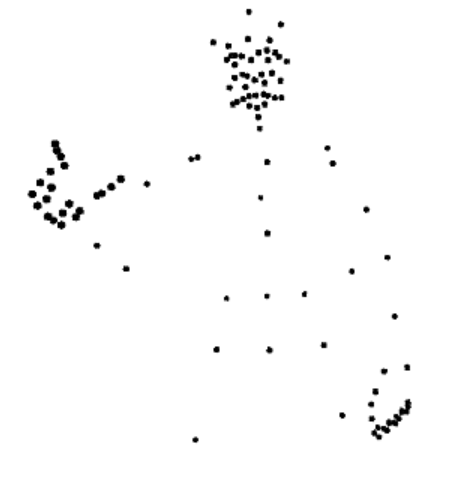
\includegraphics[width=0.34\linewidth]{Images/Johansson.png}
    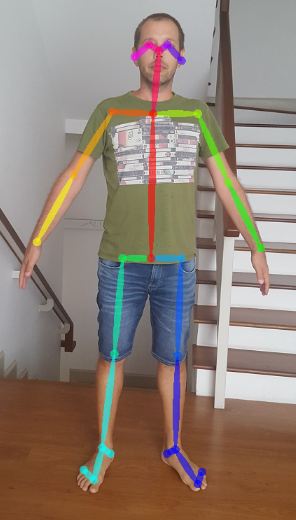
\includegraphics[width=0.2\linewidth]{Images/openpose2.png}
    \caption{A gauche: Un exemple de stimuli de l'experience de Johansson \cite{johansson1973visual,johansson1976spatio}.\\ A droite: la squelettisation obtenue après l'application d'Openpose \cite{cao2017realtime}}
    \label{fig:Johansson}
\end{figure}

Par conséquent, nous 

\textit{De ce fait, nous avons du nous intérésser à plusieurs étapes qui seront considérées comme des parties indépendantes de notre approche}


PipeLine: SQUELETTE -> HAR -> INTENTION

\subsection{Squelettisation de piétons}
La nécéssité première de cette thèse consiste donc en l'obtention d'une squelettisation cohérente de chaque piéton présent dans l'image au fil du temps.

Cette squelettisation sera ensuite utilisée en tant que donnée d'entrée de notre réseau afin d'en inférer une classe en fonction de la gestuelle de celui-ci.

La tâche de détection est compliquée par la variabilité de l’apparence des personnes (vêtements, pose ...)
ainsi que par des phénomènes d’occlusions, dûs à la foule et au décor ou encore dûs à des problèmes d'echelle dans l'image.




\label{subsec:SQUEL}
\subsubsection{Approches Top Down}
\subsubsection{Approches Bottom Up}

\subsection{Human Action Recognition}

\textbf{ Compared to RGB videos and optic flow,skeleton sequences are computationally efficient. Furthermore,skeleton  sequences  have  a  better  ability  to  represent  dataset-invariant  action  information  since  no  background  context  isincluded.
Parler des handcrafted?}

\textit{3D action recognition – analysis of human actions based on3D  skeleton  data  –  becomes  popular  recently  due  to  its  succinctness,robustness, and view-invariant representation}

La seconde étape de l'approche consistera en la classification des actions de la personne,

Les principales modalités utilisées pour la reconnaissance d'actions humaines comprennent les vidéos RGB dans leur globalité \cite{donahue2015long,2014arXiv1412.0767T,varol2017long,Wu_2018_CVPR}, le flow optique \cite{simonyan2014two,zhang2016real,sevilla2018integration,DanutPOP} et la réprésentation sous forme de squelette \cite{vemulapalli2014human,du2015hierarchical,2016arXiv160707043L,2018arXiv180107455Y}.

En réduisant la taille des données d'entrée grâce à la structure de données associée aux squelettes, ce type d'approche est considéré comme bien plus rapide computationellement parlant.

\label{subsec:HAR}

\subsubsection{Image-Based}
\subsubsection{Recurent neural network based}
\subsubsection{Graph Based}

\subsection{Intention Prediction}
\textit{La plupart des approches actuelles de la prédiction de l'action des piétons sont basées sur la trajectoire [16, 1, 5], ce qui signifie qu'elles s'appuient sur le mouvement passé observé des piétons et/ou la dynamique des véhicules pour prédire l'emplacement futur des piétons. Ces approches sont toutefois efficaces lorsque les piétons traversent déjà laa rue ou sont sur le point de le faire, c'est-à-dire que ces algorithmes réagissent à une action déjà en cours au lieu de l'anticiper.}

Un remède aux inconvénients courants des algorithmes basés sur la trajectoire est d'anticiper l'action en estimant sa cause ou son intention non déviante.


In the literature various terms such as intention, actionand behavior are used to describe what the agent is doing or about to do in the scene. Here, we distinguish intention as the underlying state of mind which cannot be observed but can be inferred from the behavior. This is opposed toactions and, more generally, behaviors, i.e. observable ac-tions such as walking or crossing, for which there is groundtruth available.




\subsubsection{Handcrafted}
\subsubsection{Apprentissage profond}




% SEC1
\input{./Sections/Section_2}

% SEC1
\clearpage
\chapter{Experimentations, Réalisations}
\label{sec:SOTA}

\section{Représentation Graphe/Squelette porteuse de sens}

\subsection{Introduction}
Le format de structure de données de la majorité des articulations disponibles via les approches de squelettisation en un tenseur ignore les relations de dépendance physique entre les articulations et ajoute de fausses connexions entre les articulations du corps qui ne sont pas liées physiquement.

\begin{figure}[H]
    \centering
    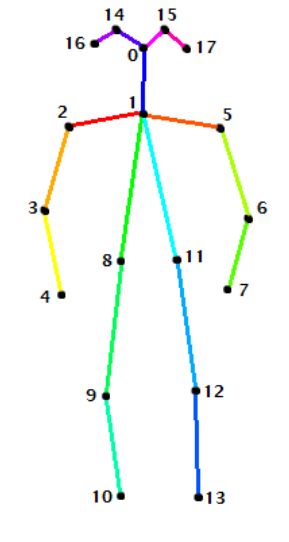
\includegraphics[width=0.3\linewidth]{Images/openpose.png}
    \caption{Structure de données de la représentation squelette obtenue à l'aide de la bibliothèque OpenPose \cite{cao2017realtime}}
    \label{fig:openPoseSkel}
\end{figure}

La figure \ref{fig:openPoseSkel}, nous permet de constater que conserver le squelette obtenu par les algorithmes de detection de pose classiques, sans avoir recours à une transformation pourrait réduire la qualité de nos résultats: certains couples d'articulations, bien que se suivant de manière incrémentale dans la structure de données utilisée, n'ont en réalité aucune raison valable de l'être: par exemple, l'extrémité gauche du bras et l'épaule droite (\textit{nodes 4 et 5}) ou encore l'extrémité droite du bras et la hanche gauche (\textit{nodes 7 et 8}).

Une grande majorité des travaux actuels semblent négliger l'importance de cette représentation spatiale et ne se focalisent que sur le coté temporel: la dynamique des articulations, sans remettre en question la structure de données spatio-temporelle en entrée.

\subsection{Méthodologie}

En reprenant les travaux de \cite{liu2016spatio} et \cite{2018arXiv180110304Y}, j'ai souhaité m'intérésser à cette question de représentation: en réalisant un Depth-First Search (DFS) sur un hub du graphe représentant le squelette. De cette manière, il est possible d'obtenir une structure de type arbre/graphe n'exploitant que des liens de voisinage entre joints existants.

\algnewcommand\algorithmicforeach{\textbf{for each}}
\algdef{S}[FOR]{ForEach}[1]{\algorithmicforeach\ #1\ \algorithmicdo}

\begin{algorithm}
 \caption{Explorer}\label{algorithm1}
 \KwIn{graphe G, sommet s}
  marquer le sommet s\;
  afficher(s)\;
 \ForEach {sommet $t$ fils de $s$}{
  \eIf{$t$ n'est pas marqué}{
    Explorer(G,t)\;
  }
 }
\end{algorithm}


\begin{algorithm}
 \caption{Depth-First Search (DFS)}\label{algorithm1}
 \KwIn{graphe G}
 %\KwOut{how to write algorithm with \LaTeX2e }
 %initialization\;
 \ForEach {sommet $s \in \mathcal G $}{
  \eIf{s n'est pas marqué}{
    explorer(G,s)\;
  }
 }
\end{algorithm}

L'exploration d'un DFS depuis un sommet $s$ fonctionne comme suit. L'algorithme poursuit  un chemin dans le graphe jusqu'à une feuille ou jusqu'à atteindre un sommet déjà visité. L'algorithme revient alors sur le dernier sommet où il était possible de suivre un autre chemin puis continue d'explorer. L'exploration s'arrête quand tous les sommets depuis $s$ ont été visités.

Ainsi, en reprenant la structure de données format tenseur d'un jeu de données, il est possible de réaliser un DFS afin d'obtenir une représentation respectant les relations de dépendance physique du squelette (\ref{fig:DFS}).

\begin{figure}[H]
    \centering
    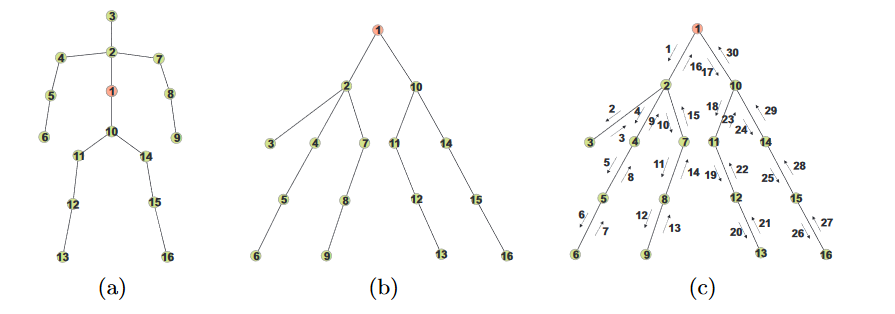
\includegraphics[width=1\linewidth]{Images/DFS.png}
    \caption{(a) Articulations du squelette d'un corps humain avec la structure de données initiale. L'ordre de visite des noeuds est incrémentale:1-2-3-...-16. (b) Le squelette est transformé en une structure arborescente. (c)  L'arbre peut être dépilé en une chaîne dont l'ordre de visite des noeuds conserve la relation physique des articulations: 1-2-3-2-4-5-6-5-4-2-7-8-9-8-7-2-1-10-11-12-13-12-11-10-14-15-16-15-14-10-1, Figure équivalente à la figure 2 dans  \cite{liu2016spatio}.}
    \label{fig:DFS}
\end{figure}

Souhaitant m'intéresser à la plus value apportée par cette représentation proposée par \cite{liu2016spatio} et \cite{2018arXiv180110304Y} pour la classification d'actions squelettiques, j'ai souhaité me comparer à un modèle de classification existant pour les mêmes conditions experimentales dans le cadre de convolutions 1D et convolutions 2D. Je me suis donc basé sur l'approche experimentale de Double-feature Double-motion Network \cite{2019arXiv190709658Y} ainsi que sur leur architecture présentée en \ref{fig:DDnet} pour les CNN 1D et avec un simple modèle convolutifs pour les convolutions 2D.


\begin{figure}[H]
    \centering
    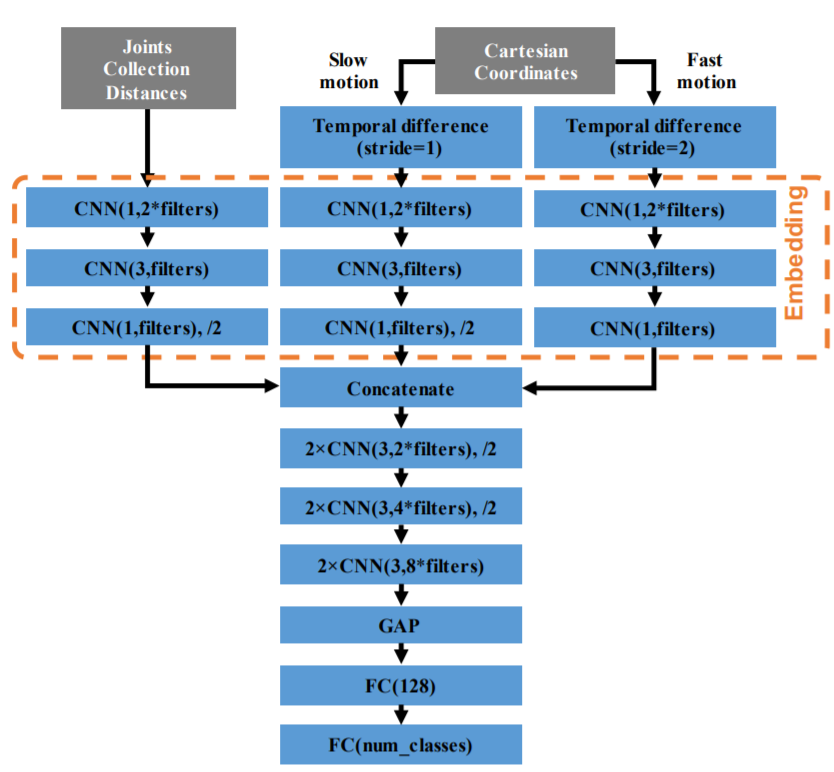
\includegraphics[width=0.55\linewidth]{Images/ddnet.png}
    \caption{L'architecture du réseau DD-Net. \textit{2×CNN(3,
2*filters),/2} désigne deux couches 1D ConvNet (taille du noyau
= 3, channels = 2*filtres) et un Maxpooling (strides = 2).GAP
désigne le Global Average Pooling. FC signifie "Fully Connected". La taille du modèle est ajustable en fonction de la variable \textit{filters}.}
    \label{fig:DDnet}
\end{figure}

\subsection{Tests et évaluations}
\subsubsection{Evaluation datasets et protocole d'évaluation}
Nous avons expérimenté les capacités de cette représentation sur deux jeux de données de reconnaissances d'action squelettiques: SHREC (actions de la main en 3D) proposé par \cite{de2017shrec} et JHMDB (action du corps en 2D)  proposé par \cite{jhuang2013towards}.\\

Simlairement à \cite{2019arXiv190709658Y} mais par manque de temps, SHREC est évalué pour un des deux cas : pour 14 gestes. L'ensemble de données JHMDB est évalué en utilisant des squelettes annotés manuellement, et l'évaluation se fait par cross-validation sur un split 3.

\subsubsection{Détails d'implémentation}
\subsubsection{Modèle CNN 1D}
L'entrainement se réalise sur une RTX 2080 Ti, les conditions experimentales ne diffèrent pas de \cite{2019arXiv190709658Y}.

\subsubsection{Modèle CNN 2D}


\subsubsection{Résultats et discussion}


\begin{table}[H]
\centering
\scalebox{0.95}{
\begin{tabular}{l|l|l|l} 
\hline
\textbf{Méthode}               & \textbf{Paramètres} & \textbf{14 classes} & \textbf{28 classes}  \\ 
\hline
DD-NET (64 filtres)     & 1.82M               & 94.6\%              & 91.9\%               \\
DD-NET (32 filtres)     & 0.50M               & 93.5\%              & 90.4\%               \\
DD-NET (16 filtres)     & 0.15M               & 91.8\%              & 90.0\%               \\ 
\hline
DFS-DD-NET (64 filtres) & 1.84M               & 95.9\%              &                      \\
DFS-DD-NET (32 filtres) & 0.51M               & 94.7\%              &                      \\
DFS-DD-NET (16 filtres) & 0.16M               & 93.1\%              &  90.5\%                   
\end{tabular}
}
\caption{Résulats obtenus grâce à la normalisation DFS sur SHREC \cite{de2017shrec} (Squelettes de main 3D)}
\end{table}

\begin{table}[H]
\centering
\scalebox{0.85}{
\begin{tabular}{l|l|l}
\textbf{Méthode}       & \textbf{Paramètres} & \textbf{Resultats}  \\ 
\hline
Chained Net \cite{2017arXiv170400616Z}             & 17.5M           & 56.8\%              \\
EHPI \cite{ludl2019simple}                   & 1.22M           & 65.5\%              \\
POTION    \cite{choutas2018potion}              & 4.87            & 67.9\%              \\
DD-Net (filters 64)     & 1.82M           & 77.2\%              \\
DD-Net (filters 32)     & 0.5M            & 73.7\%              \\
DD-Net (filters 16)     & 0.15M           & 65.7\%              \\ 
\hline
DFS-DD-NET (filters 64) & M               & \%                  \\
DFS-DD-NET (filters 32) & M               & \%                  \\
DFS-DD-NET (filters 16) & 0.15M           & 66.4\%                 
\end{tabular}}
\caption{Résulats obtenus grâce à la normalisation DFS en conservant l'architecture  \cite{2019arXiv190709658Y} sur JHMDB \cite{jhuang2013towards} (Squelettes corps humain 2D)}
\end{table}



\section{Autoencodeur semi-supervisé pour l'action recognition}

\subsection{Introduction}
Les auto encodeurs étant une composition de transformation non linéaires en esperant trouver une représentation dans l'espace adaptée au format des données et conservant un maximum de sémantique de celui-ci.

Je me suis intéréssé à cette question de représentation pour plusieurs raisons:
\begin{itemize}
    \item Tout est une question d'embedding et de normalisation en machine learning. Au final, le role premier des couches cachées est de transformer cet embedding en espérant qu'il soit porteur d'information. Le jour où l'on trouve un moyen de normaliser et de représenter les données de manière plus adequate, n'importe quel classifieur pourra obtenir de bons résultats pour peu que les données d'entrée soient porteuses d'information. Le jour ou l'on arrivera à obtenir une représentation utilisable plus rapidement au lieu de stacker des layers au sein d'un réseau de neurones, d'autres problématiques d'apprentissage apparaitront mais le gain serait intéréssant: (Selon le théorème d'approximation universelle, n'importe quel Shallow Network peut supposément approximer une fonction donnée \cite{universalapproxtheorm,scarselli1998universal}).
    
    \item En s'intéréssant à la question de la représentation des données, on évite un apprentissage de cette représentation à "l'aveugle" (en optimisant un réseau précis sur un jeu de données précis et en testant un maximum d'hyperparamètres on est assurés de faire un bon résultat.  On peut potentiellement réduire la taille de notre réseau et donc par définition réduire le temps d'inférence de celui-ci, ce qui peut être intéréssant dans le cadre d'un sujet en temps réel.
\end{itemize}

L'idée étant d'entrainer un autoencodeur avec une fonction de coût modifiée en rajoutant une contrainte sur la séparation linéaire des classes dans l'espace latent (LDA / QDA / FDA). Il a été montré que la représentation optimale interne d'un MLP s'obtient en faisant une analogie avec une analyse discriminante non linéaire \cite{webb1990optimised}.

Les approches factorielles citées plus haut s'apparentent à la projection de données dans l'espace comme celle d'une ACP mais tandis que l'ACP maximise la variance du jeu de données, celles-ci se focalisent sur la maximisation de la séparabilité des classes dans l'espace (supervisé). On obtiendrait donc un AutoEncodeur "semi-supervisé" dans le sens où celui-ci se focalise sur deux informations complètement différentes dans les données, l'une de manière non-supervisée, l'autre de manière supervisée:
\begin{itemize}
    \item La structure inhérente des données capturée de manière non supervisée grâce à l'Auto-encodeur, on conserverait une partie de l'information importante et discriminante du jeu de données. (feature extraction)
    \item La séparabilité des classes dans l'espace grâce à l'analyse discriminante (non) linéaire. Ce qui permettrait de réduire le nombre de layer au final.
\end{itemize}{}


Une fois la convergence obtenue, on peut imaginer deux utilisations:
\begin{itemize}
    \item Récupérer cet espace latent combinant les informations "data driven" grâce à l'apprentissage non-supervisé de l'auto encodeur classique et une première ébauche de séparabilité linéaire grâce à la seconde partie de la fonction de coût. Envoyer l'espace latent à un input de CNN classique très peu profond, GAP, Softmax ou un MLP, Softmax. Finetuner le réseau de bout en bout et voir ce que cela donne quand à la capacité de discrimination de l'approche. 
    \item Générer des données en réalisant une génération d'instance au niveau de l'espace latent grâce à des approches type SMOTE \cite{chawla2002smote} ou ADASYN \cite{he2008adasyn}  et utiliser la partie décodeur pour  faire de la data génération.
\end{itemize}

\subsection{Formalisation}
On pose le problème comme ceci: \newline
$$\min _{\theta_{1}, \theta_{2}},\left\|\mathbf{X}-g_{\theta_{2}}\left(f_{\theta 1}(\mathbf{X})\right)\right\|^{2}$$

Fonction de coût habituelle d'un autoencodeur avec $\theta_{1}, \theta_{2}$ les paramètres des blocs encodeur et decodeur de l’AE. 

$$\min _{\theta_{1}, \theta_{2}, \mathbf{S}}\left\|\mathbf{X}-g_{\theta_{2}}\left(f_{\theta_{1}}(\mathbf{X})\right)\right\|^{2}+\lambda\left\|f_{\theta_{1}}(\mathbf{X})-\mathbf{S}_{f_{\theta 1}}(\mathbf{X})\right\|^{2}$$

Ajout d'une variation dans la fonction de coût: avec S la matrice de projection des individus dans l'espace latent obtenue avec une analyse discriminante linéaire (LDA) et $\lambda$ un régularisateur.

Une fois, l'entrainement de l'autoencodeur réalisé, récupération des poids de la partie encodeur: $f_{\theta 1}$, ajout d'une fonction classifieur softmax:\\ 

$\sigma(\mathbf{z})_{j}=\frac{\mathrm{e}^{z_{j}}}{\sum_{k=1}^{K} \mathrm{e}^{z_{k}}} \text { pour  tout } j \in\{1, \ldots, K\}$


\begin{figure}[H]
    \centering
    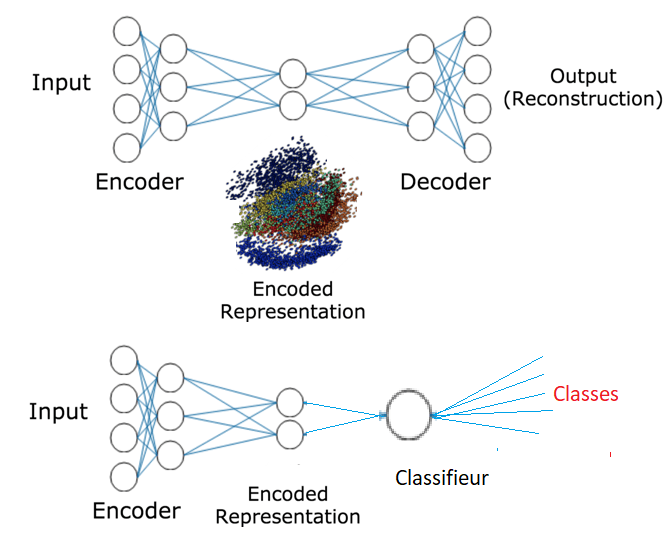
\includegraphics[width=0.8\linewidth]{Images/Autoencoder_modif.png}
    \caption{Pipeline de l'approche}
    \label{fig:AEmodif}
\end{figure}

\subsection{Tests et évaluation}
J'ai réalisé l'implémentation de cette approche sur deux jeux de données: SHREC \cite{de2017shrec} et JHMDB \cite{jhuang2013towards}.\\

\begin{table}[H]
\centering
\scalebox{0.75}{
\begin{tabular}{l|l|l|l|l}
\hline
\textbf{Méthode}                                 & \textbf{Nb Params} & \textbf{SHREC 14} & \textbf{SHREC 28} & \textbf{FPS (RTX 2080 ti)}  \\ 
\hline
LDA sur l'input                   &          - &         33.0\% &          27.6\%&      \\
LDA sur le bottleneck AE classique (\lambda = 0)              &          - &         37.9\% &          42.8\%&      \\
LDA sur le bottleneck AE modifié (\lambda = 5)              &          - &         43.5\% &          35.6\%&      \\
\hline
MLP Sans initialisation                      &          1.2M &         91.2\% &          85.2\%&     20 000 \\
MLP Avec initialisation AE classique (\lambda = 0)        &          1.2M &          91.5\%&          85.9\%&      -\\
MLP Avec initialisation AE Modifié (\lambda =1) &          1.2M &          91.9\%&          87.6\%&      -\\
MLP Avec initialisation AE Modifié (\lambda = 2.5) &           1.2M&          92.4\%&          86.9\%&     -\\
MLP Avec initialisation AE Modifié (\lambda = 5)          &          1.2M &          \textbf{92.5\%}&         \textbf{87.1}\% &      -\\
MLP Avec initialisation AE Modifié (\lambda = 7.5) &          1.2M &         91.9\% &          86.4\%&      -\\
MLP Avec initialisation AE Modifié (\lambda = 10) &          1.2M &          90.9\%&          85.2\%&      -


\end{tabular}}
\caption{Résulats obtenus grâce à l'initialisation des poids avec un AE modifié sur SHREC \cite{de2017shrec}}
\end{table}




\begin{table}
\scalebox{0.7}{
\centering
\begin{tabular}{l|l|l|l} 
\hline
\textbf{Methode}                  & \textbf{Nb Params} & \textbf{\textcolor[rgb]{0.129,0.145,0.161}{Average accuracy of 3 splits ~})\textcolor[rgb]{0.129,0.145,0.161}{}~} & \textbf{Classifications par secondes}  \\
\hline
Chained Net (ICCV17)              & 17.50 M            & 56.8\%                                                                                                                                        & 33 (1080 Ti)                           \\
EHPI~ (ITSC19)                    & 1.22 M             & 65.5\%                                                                                                                                        & 29 (1080 Ti)                           \\
PoTion (CVPR18)                   & 4.87 M             & 67.9\%                                                                                                                                        & 100 (1080 Ti)                          \\
DD-Net                            & 1.82M              & 77.2\%                                                                                                                                        & 2,200 (1080 Ti)                        \\ 
\hline
Sans initialisation (\lambda =0)~ & 0.67M                  &   65.2\%                                                                                                                                            & -                                      \\

Avec initialisation AE classique (\lambda =0)~ & 0.67M                  &   66.4\%                                                                                                                                            & -                                      \\
Avec initialisation AE modifié (\lambda =1)    & -                  &          66.2\%                                                                                                                                     & -                                      \\
Avec initialisation AE modifié (\lambda =2.5)   & -                  &          68.3\%                                                                                                                                     & -                                      \\
Avec initialisation AE modifié (\lambda =5)   & -                  &        67.9\%                                                                                                                                       & -                                      \\
Avec initialisation AE modifié (\lambda =7.5)   & -                  &          66.5\%                                                                                                                                     & -                                      \\
\hline
\end{tabular}}
\end{table}

\begin{figure}[H]
    \centering
    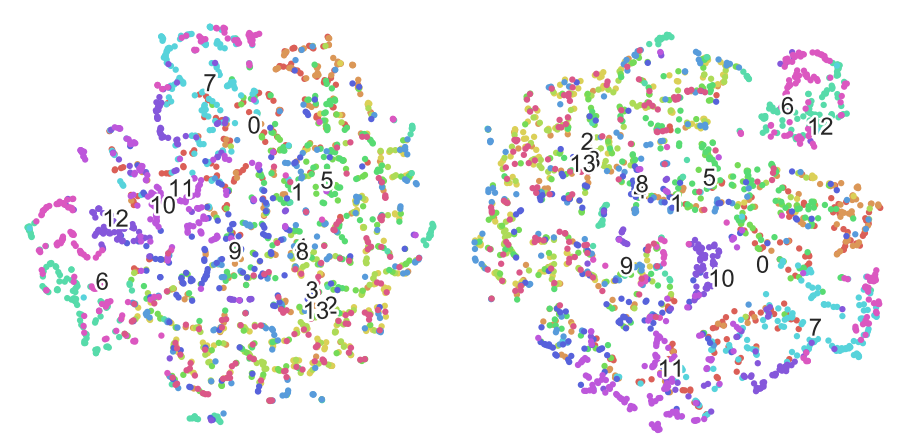
\includegraphics[width=0.8\linewidth]{Images/tsne_results.png}
    \caption{Visualisation des espaces latents via T-Sne: à gauche auto-encodeur classique, à droite auto-encodeur modifié ($\lambda$ = 10)}
    \label{fig:AEmodifTSNE}
\end{figure}

\begin{figure}[H]
    \centering
    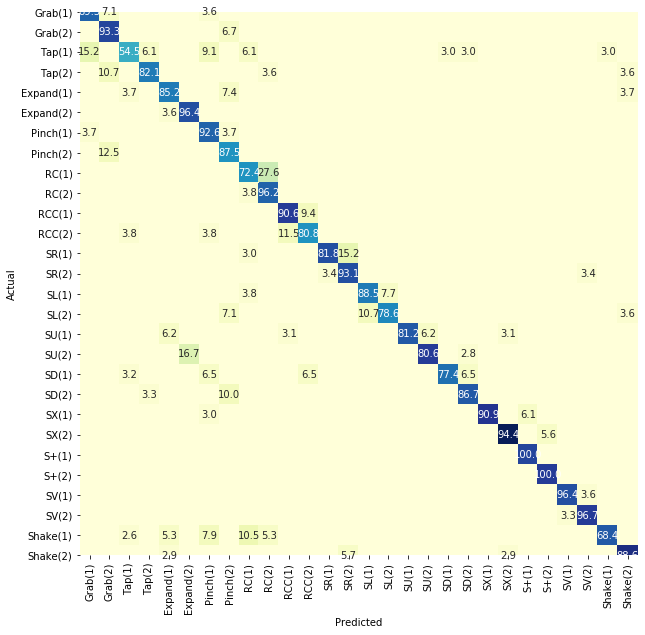
\includegraphics[width=0.8\linewidth]{Images/shrec28.png}
    \caption{ca}
    \label{fig:rsshrec28}
\end{figure}\textbf{}

\subsection{Remarques}
\begin{itemize}
    \item Le nombre maximum d'axes obtenus par la LDA correspond au nombre de classe moins un: sur SHREC 14 l'espace latent est donc de dimension 13 toute représentation avec un espace latent superieur est impossible (on ne peut donc difficilement imposer des contraintes de sparsité au modèle). Cela implique également une perte très lourde de l'information vis-à-vis de l'information dans l'espace latent. (SHREC: de 2122 neurones d'entrée à un espace latent avec 13 neurones)
    \item Quelques problèmes de convergence dûs à l'optimisation de $\lambda$ durant l'apprentissage de l'autoencodeur avec la fonction de coût modifiée(optimiser ADAM \cite{kingma2014adam}).
\end{itemize}

\subsection{A creuser}

Essayer plusieurs structures plus travaillées qu'un simple MLP:
\begin{itemize}
    \item AE: Convolutions / Attention / Séquentiel / VAE.
    \item analyse discriminante: QDA  pour ne pas émettre de suppositions vis-à-vis des matrices de covariance de chaque classes
\end{itemize}

Rien n'est fixé dans la fonction de coût, j'imagine qu'ajouter un autre critère de régularization ne peut être que bénéfique, mais vu les prolèmes de convergence actuels, je préfère ne pas le tenter pour l'instant.




% SEC1
\input{./Sections/Section_4}

% SEC1
\clearpage
\section{Démarche proposée au cours de la thèse}
\label{sec:SOTA}

\subsection{Bases de données}

\subsection{Idées}

% SEC1
\clearpage
\chapter{Conclusion}
\label{sec:SOTA}

Au cours de ces huit mois de thèse, un état de l'art a été effectué pour plusieurs domaines de recherche dans l'optique de les combiner sous la forme de briques indépendantes afin de répondre à la problématique actuelle du sujet de thèse : «Peut-on lier la dynamique des articulations d'un piéton à une intention ? »\\


\textbf{L'estimation de pose}, nécessaire étape d'une prédiction dont l'analyse de la posture est un composant essentiel. Nous avons présenté les deux types d'approches pour la squelettisation: Bottom up et Top Down. La robustesse des approches Top Down comparé aux approches Bottom up et la capacité à pouvoir minimiser leur temps d'inférence dans le cadre spécifique de nos travaux nous pousse à sélectionner une méthode de l'état de l'art de ce type afin de squelettiser les piétons. Nous avons ensuite étudié les questions relatives à la dimension du squelette obtenu et l'utilisation des informations séquentielles pour obtenir une meilleure inférence. Tandis que les approches de squelettisation 3D sont moins abouties de par la faible quantité de jeux de données annotés, la recherche sur la question de la séquentialité pour l'estimation de pose semble plus aboutie. Nous avons donc pour l'instant décidé de nous focaliser sur une approche Top Down prenant en compte la séquentialité à base d'appariement de pose. Cela afin de pouvoir réaliser un meilleur suivi des protagonistes de la scène et de ne pas mélanger les dynamiques de deux protagonistes probablement du à un changement d'angle de caméra. A plus long terme, il est néanmoins envisagé d'adapter une approche de l'état de l'art de ce type afin de l'associer à un modèle d'inférence 3D pour régler des problèmes que nous pourrions rencontrer tels que les problèmes d'occlusion dans une scène bondée.   \\


\textbf{La reconnaissance d'actions squelettiques}, afin d'obtenir une idée générale des types d'approches utilisés dans l'état de l'art pour ce format de donnée. Comparé aux approches dites classiques d'apprentissage profond pour le traitement de données séquentielles, les convolutions semblent toutes aussi légitimes quand à leur utilisation pour cette tache. De plus, leur capacité à converger plus vite et à pouvoir traiter des entrées de longueur variable en fait une approche de choix dans le cadre de nos travaux où la vitesse d'inférence est importante. Il est intéressant de constater que la majorité des approches semblent minimiser l'importance de la cohérence d'une structure de données spatio-temporelle respectant les relations de dépendance physique. Par conséquent, nous souhaitons actuellement axer notre recherche dans ce domaine et construire une représentation de l'information permettant une justification du conditionnement des réseaux et une explicabilité des résultats conservant ces relations de dépendance physique. Que cela soit en utilisant une normalisation en entrée sur les données ou en utilisant de l'attention dite spatiale, afin d'aider le réseau de neurones à sélectionner, ou à pondérer différemment, les parties du corps avant d'analyser les évolutions temporelles des articulations. \\


\textbf{La prédiction d'intention}, laissant apparaître d'autres problématiques comparé à la reconnaissance d'actions seule : la nécessité de réaliser une inférence sur une séquence incomplète. Nous distinguons deux types de prédiction: continue et discrète (à court et long terme). Tandis que les inférences à long terme sont un aspect qui ne sera pas approfondi d'avantage de par la nature de nos travaux sur des séquences assez courtes, le conditionnement des actions en fonction d'un objet présent dans la scène peut-être une piste à approfondir pour améliorer la qualité du modèle.
L'inférence à court terme d'une action peut être traitée de plusieurs manière: ajouter une contrainte à la fonction de coût du réseau pour prioriser les premiers pas de temps ou utiliser sur des méthodes génératives de l'état de l'art. Nous allons pour l'instant prioriser la première approche afin de ne pas alourdir le temps d'inférence du modèle car l'adaptation d'une fonction de coût n'influencera en rien le temps d'inférence d'un modèle comparé aux méthodes génératives qui peuvent être gourmandes en temps de calcul. Cela afin de conserver à l'esprit la contrainte majeur de notre travail: la contrainte temps réel.
Nous nous orientons donc notre recherche vers la création d'une architecture de traitement via réseaux de neurones multimodales prenant en charge des dynamiques à périodes courtes ainsi que des méta-informations supplémentaires en entrée. L'approche pour l'inférence continue sera par exemple conditionnée en ajoutant la classe discrète d'action du piéton sous la forme d'une méta information au même titre que d'autres données mixtes (squelette, image, informations qualitatives: contexte) avec une fonction de coût modifiée pour prioriser les premiers pas de temps et classifier correctement l'action le plus rapidement possible. \\


%%%%%%%%%%%%%%%%%%%%%%%%%%%%%%%%%%%%%%%%%%%%%%%%%%%%%%%%%%%%%
%APPENDICES
%%%%%%%%%%%%%%%%%%%%%%%%%%%%%%%%%%%%%%%%%%%%%%%%%%%%%%%%%%%%%


\appendix
\renewcommand*{\thesection}{\Alph{section}}\textbf{}

% APPENDIX A
\clearpage
\section{Appendix}
\label{app:A}






%%%%%%%%%%%%%%%%%%%%%%%%%%%%%%%%%%%%%%%%%%%%%%%%%%%%%%%%%%%%%
%BIBLIOGRAPHY
%%%%%%%%%%%%%%%%%%%%%%%%%%%%%%%%%%%%%%%%%%%%%%%%%%%%%%%%%%%%%

\clearpage
\renewcommand*{\thesection}{}\textbf{}

\bibliographystyle{plain}
\bibliography{Bibliography.bib}


\end{document}